\documentclass[12pt]{article}
\usepackage{titlesec}
\usepackage{setspace}
\usepackage{graphicx} 
\usepackage{color}
\usepackage[left=1.5in,top=1in,right=1in,bottom=1in]{geometry}
\textwidth 6in
\textheight 9in
\parskip 7.2pt           % sets spacing between paragraphs
\parindent 0pt		 % sets leading space for paragraphs
\titleformat{\section}{\bfseries}{\thesection}{12pt}{}
\newcommand{\sectionbreak}{\clearpage}
\begin{document}         
% Start your text

%\color{blue}

\begin{center}
\break \break \break \break 
Artificial Plasticity: Measuring The Effect of Greedy, Layer-Wise Pre-Training on Visual-Auditory Generalization of Denoising Autoencoders
\break\break\break\break \break \break \break \break \break 
by \break \break Nathan H. Nifong
\break\break\break\break \break \break \break \break \break 
A thesis submitted in partial fulfillment of the\break
requirements for the degree of
\break\break\break\break 
Master of Science \break in \break Systems Science
\break\break\break\break \break 
Thesis Committee: \break Wayne Wakeland, \break Marty Zwick, \break Melanie Mitchell.
\break\break\break\break 
Portland State University \break 2013
\end{center}

\begin{singlespacing}
\tableofcontents
\end{singlespacing}

\section{Abstract}
\label{Abstract}
\begin{doublespacing}

One of the most impressive qualities of the brain is it's neuro-plasticity. The neocortex has roughly the same structure throughout it's whole surface, yet it is involved in a variety of different tasks from vision to motor control, and regions which once performed one task, can learn to perform another \cite{hawkins2004intelligence}. Machine learning algorithms which aim to be a plausible model of the neocortex should also display this plasticity. One such candidate is the stacked denoising autoencoder (SDA). It has shown promising results in the field of machine perception where it has been used to learn abstract features from unlabeled data. \cite{larochelle2007empirical, le2011building, vincent2008extracting} In this thesis I develop a flexible distributed implementation of an SDA and train it on images and audio spectrograms to experimentally determine properties comparable to neuro-plasticity, Specifically, I compare the visual-auditory generalization between a multi-level denoising autoencoder trained with greedy, layer-wise pre-training (GLWPT), to one trained without. Networks pre-trained on one sensory modality performed [better] on the other modality than randomly initialized networks trained for an equal total number of epochs. Furthermore, the magnitude of improvement gained from this pre-training is [greater] when GLWPT is applied, than when it is not, leading to the conclusion that the GLWPT training helped the SDAs learn abstract features, and this in turn improved it's generalizability between different sensory modalities. 

\section{Introduction and Background}

	\subsection{Neural Plausibility of Machine Learning Algorithms}
		The latest strides in the field of machine learning are coming from deep networks \cite{hinton2012deep, lee2009convolutional, grubb2010boosted, tang2012deep, krizhevsky2012imagenet, bengio2009learning}. This class of learning algorithm is inspired by the structure of the mammalian neocortex, specifically the visual areas in the occipital lobe which have been studied more extensively than any other part. This is in contrast to the non-neurally inspired algorithms such as support vector machines  (SVM) that are more widely used and were notably better at classification than neural networks. %citation here, who says the algorithms are really more widely used.
Now that we are seeing biologically inspired algorithms leading the way, biological plausibility becomes a useful heuristic for the further development of algorithms with higher performance measures, and discoveries about the emergent properties of these algorithms may feed back into neuroscience to inform further study of the brain. 
		One metric which defines the brain and differentiates it from other intelligent systems is it's plasticity. Areas which once specialized in a certain function can change and learn a new function if for some reason they cannot continue with their first function or if the second function is just much more demanding of computational resources. \cite{sharma2000induction}
		
	\subsection{Hierarchical representation in the brain}
		Deep networks are like the neocortex in many ways, but the most important of them is the hierarchical structure from which they get their name. In the visual cortex, neuroscientists have found using single-neuron recording that there are cells which respond most strongly to specific visual stimuli. The nature of the stimuli which excite the neurons changes changes along many dimensions throughout the visual cortex. One of the more salient dimensions of variation is that of \em abstraction\em\cite{hinton2005kind}. The organization of the visual cortex is illustrated in figure ~\ref{fig:visualcortex}. The cells in V1 are the first cells in the cortex to receive signals from the retina via the lateral gesticulate nucleus, a part of the thalamus. Cells here respond most actively to a particular edge at a particular angle within a small area of vision called their receptive field. As one moves up V2, V3, V4, and V5 the cells respond to more and more abstract visual stimuli until one sees cells that do things like activating whenever a dog is in the visual field, when objects appear to be moving in a specific way, and even abstract visual conditions such as "currently looking at object in hand" regardless of what or where it is. While it is possible that each of those abstract stimuli has a large set of neurons dedicated to recognizing it out of a "raw" sensory stream, it's far more plausible that they recognize it out of a small, and information-rich stream of intermediate representations, Leading to the idea that a hierarchical structure is crucial to the functionality of the neocortex.
		
\begin{figure}[p]
\centering
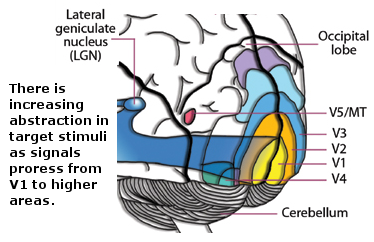
\includegraphics[scale=0.8]{visual_cortex}
\caption{An Illustration of the areas within the visual cortex. The layers in a deep networks mimic the stages of processing in the visual cortex. From \em On The Origin Of The Human Mind \em by Andrey Vyshedskiy}
\label{fig:visualcortex}
\end{figure}
		
	\subsection{The reusability of hierarchical representations.}
	A hierarchical, or tree-like structure of knowledge representation allows one to construct compact representations of a massive and complex distribution of stimuli. First one learns that the data can be represented in a slightly more compact way as a finite collection of simple patterns corresponding to local, high-frequency (short-term), salient features in sensory signals. A similar process is applied to the first-level features to construct another set of more abstract features, which can represent the data even more compactly. Thus, one re-uses representations rather than learning a whole new set for each abstract feature.
	In the case of vision, the levels of a hierarchy of representation might be as follows. Images can all be represented as pixel arrays, And pixel arrays can be represented more compactly as a collection of overlapping gradients, edges, and spots chosen from a finite set, and colored with a small finite set of colors. (this is the principle behind JPEG compression and appears to be the principle organization of the visual striate cortex.) These patches, are commonly compared to Gabor filters %cite something about Gabor filters
, depicted in figure ~\ref{fig:gaborz}, and are the most commonly learned set of features in machine vision. As one moves up the chain of abstraction in vision, nearly all combinations of edges and spots seen in natural images can be represented even more compactly as a hierarchy of things, stuck to the surfaces of bigger things in roughly specified locations, illuminated from a given angle \cite{gluckman2003kurtosis}. Assuming you have a library of hundreds of thousands of things, and the texture of spots, edges, and colors that typically make up their surface, and the ability to calculate shadows, one can decode, or render this representation into the one below it.

\begin{figure}[p]
\centering
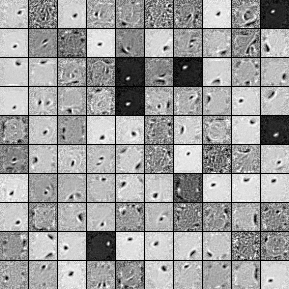
\includegraphics[width=4in,height=4in]{filters_corruption_30}
\caption{Edge, spot and gradient filters learned by a single denoising autoencoder. These are a common and efficient first level feature set for natural images. A feature is actually a set of weights, but an image can be generated to represent it, corresponding to the inputs that would produce a full signal on the given feature, and zero signal on all others. The extent to which these features resemble theoretical Gabor filters is an indicator of how well the model has generalized.}
\label{fig:gaborz}
\end{figure}
	
	The tricky part of course is learning the vocabularies of symbols that make up each layer and the weights on the connections that allow you to translate between them. Traditional multi-layer neural networks assume pre-set finite number of layers, and nodes at each layer, and then attempt to learn the feed-forward weights which connect layers  all at once using back-propagation and Stochastic Gradient Descent (SGD). There are no weights which operate on the information feeding backwards except in some recurrent neural networks. For the most part, pure SGD doesn't work very well. On large networks (hundreds of nodes at each layers and more than 3 layers) the search will get stuck in effective local minima. %cite here. who says multilayer networks get stuck?
	
	\subsection{Deep networks}
Deep networks can have the same structure as traditional neural networks (set number of layers, set number of nodes at each layer, full feed-forward connections, and sigmoid activation function) but they are trained one layer at a time in order to initialize SGD in a good basin of attraction, and they usually employ some kind of dropout in order to enforce sparse hierarchical representations\cite{hinton2012improving, krizhevsky2012imagenet}. 
% Explain what it means to be in a good basin of attraction 
Deep networks have been shown to be able to learn the abstract feature sets that traditional multi-layer neural networks were originally expected to be able to learn. There are several types of deep belief networks, but they share the property of having layers. They consist of a stack of modules, which can be increased in depth indefinitely. De-noising autoencoders, and Boltzmann machines are commonly used modules. 
% cite here one boltzmann machines and autoencoders as common modules for deep nets
For each type of module, there are many variants that differ in the method used to learn the parameters, such as marginalized autoencoders, which are optimized for speed \cite{chen2012marginalized}. In order to use a module within a deep network, the module must meet some criteria. It must perform some limited form generalization, and must operate on the same format of data it produces, such that it can be stacked recursively. So far, most modules are feed forward only. They perform inference using only the data from the layer below, but deep networks constructed of modules which operate on information passing in both directions promise to be an interesting area of research.

	\subsection{Stacked denoising autoencoders}
The aim of the autoencoder to learn the code $\mathbf y$, a distributed representation that captures the coordinates along the main factors of variation in the data (similarly to how principal component analysis (PCA) captures the main factors of variation in the data). Because $\mathbf y$ is viewed as a lossy compression of $\mathbf x$, it cannot be a good compression (with small loss) for all $\mathbf x$, so learning drives it to be one that is a good compression in particular for training examples, and hopefully for others as well, but not for arbitrary inputs. That is the sense in which an autoencoder generalizes: it gives low reconstruction error to test examples from the same distribution as the training examples, but generally high reconstruction error to uniformly chosen configurations of the input vector.

If there is one linear hidden layer (the code) and the mean squared error criterion is used to train the network, then the  hidden units learn to project the input in the span of the first  principal components of the data. If the hidden layer is non-linear, the autoencoder behaves differently from PCA, with the ability to capture multi-modal aspects of the input distribution. The departure from PCA becomes even more important when we consider stacking multiple encoders (and their corresponding decoders) when building a deep belief network \cite{hinton2006reducing}.

The autoencoder alone is not sufficient to be the basis of a deep architecture because it has a tendency towards over-fitting, and for a while restricted Boltzmann machines were clearly superior. The denoising autoencoder (dA) is an extension of a classical autoencoder introduced specifically as a building block for deep networks\cite{vincent2008extracting}.  It attempts to re-construct a corrupted version of the input, but the error in $\mathbf z$ is still compared against the un-corrupted input. This is known as "dropout" The stochastic corruption process consists in randomly setting some of the numbers in the input vector (as many as half of them) to zero. Hence the denoising autoencoder is trying to predict the corrupted (i.e. missing) values from the uncorrupted (i.e., non-missing) values, for randomly selected subsets of missing patterns. This modification allows the dA to generalize well and produces compounding benefits when the dA's are stacked into a deep network\cite{hinton2006reducing}. Geoffrey Hinton suggests that the stochastic timing of the action potentials observed in biological neurons is a similar feature evolved to moderate the potential for over-fitting, and allow neurons or neuron groups to generalize well over the range of activation patterns of their receptive fields.
	
Stacked denoising autoencoders, canonically abbreviated SDA, are not just neural networks with additional hidden layers, but a structure with individual levels of simple three-layer denoising autoencoders. First, a single denoising autoencoder is trained on the data. It's hidden layer converges on a sparse distributed representation of the training set. This essentially replaces the step where a researcher would have to design a collection of good features. Then, a second denoising autoencoder is trained to reconstruct corrupted versions of the activation of the hidden layer of the first dA for the collection of training examples. (the first level does not learn during this time). After a sufficient number of levels have been added, if the network is to be used for classification, the encoders and decoders from each level are assembled into one long network and fine-tuned using back-propagation and SGD.

\begin{figure}[p]
\centering
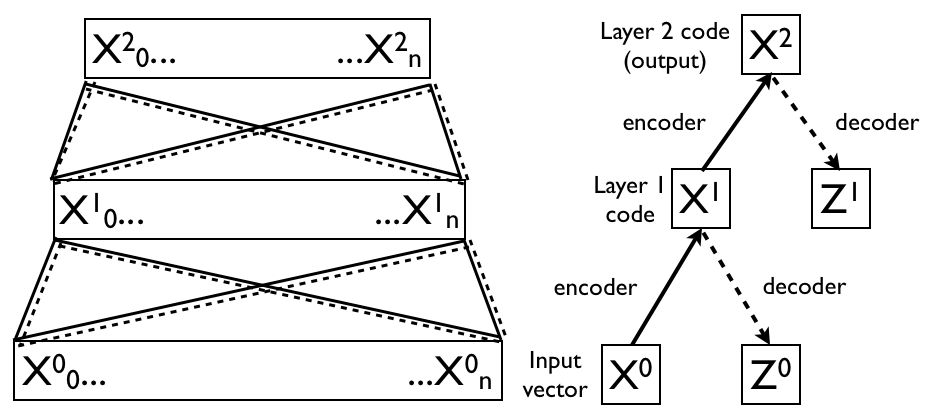
\includegraphics[width=6in]{sda_fig_}
\caption{Stacked denoising autoencoder. On the left, each layer's input is shown, with fully connected weights between them. solid lines represent encoder weights and dashed lines represent decoder weights. Levels typically become smaller as you move up the stack. On the right, each autoencoder's structure is represented. The hidden layer of each autoencoder is used as the input for the autoencoder above. }
\end{figure}

	\subsection{Relevant work}
	Brandon Rohrer at Sandia National Laboratories developed a model which learned abstract features from images and audio known as BECCA. It is inspired by the properties of the visual cortex, and attempts to re-create it's generality and flexibility. He postulates that abstract feature discovery may be responsible for the generality and flexibility of the neocortex, but that we don't yet know for certain.
\begin{quote}
\singlespacing
\em Re-routing sensory inputs to a new cortical location results in similar feature creation phenomena, hinting that the cortex may be performing a similar function throughout its extent. If that is the case, the function it performs may be nothing more than feature creation. However, there is still far too little data available to certify or disprove such a statement.\cite{rohrer2011biologically}
\end{quote}

Honglak Lee et. al. applied convolutional deep belief networks to audio classification with notable success. They extracted features from spectrograms of short audio snippets of speech from the TIMIT phoneme dataset, and from music. They were able to perform classification of the artist and the genre of songs, as well as classify phonemes from speech snippets, using the same set of learned features.\cite{lee2009unsupervised}

Undoubtedly, the most successful applications of deep networks are in the field of machine vision. One example that stands out is the classification of objects from the enormous ImageNet dataset using convolutional deep belief nets by Alex Krizhevsky, Ilya Sutskever, and Geoffrey E. Hinton\cite{krizhevsky2012imagenet}. Although they did not perform any unsupervised pre-training, they achieved record breaking classification performance. They also describe the challenges posed by distributing their computation across multiple GPUs.

Dumitru Erhan at. all have investigated why unsupervised pre-training helps stacked denoising autoencoders, and have found that unsupervised pre-training initializes a deep architecture in a basin of attraction of gradient descent corresponding to better generalization performance. They hypothesize that due to the non-convexity of the training criterion, early examples have a disproportionate influence on the outcome of the training procedure. Even so, it is still somewhat unclear why that should be the case. \cite{erhan2010does}

While there has been much research into the strengths and applications of deep belief networks and stacked denoising autoencoders specifically, there does not appear to have been any experiment to investigate the effect of unsupervised pre-training on cross-modal generalization performance of DBNs or SDAs.

	
\section{Experimental design and implementation}
	\subsection{Datasets}
	The image dataset comes from the MIRFLICKR-1M collection of 1 million images from Flickr, all licensed under Creative Commons by their original authors. Flickr credits the authors on the MFLICKR description page. 32 by 32 pixel normalized greyscale patches were desired, but at the standard 4 megapixel resolution of the example images, 32 by 32 pixel patches are smooth and relatively featureless, so 100 by 100 pixel patches were randomly sampled from the images in dataset and resized using bilinear interpolation to 32 by 32 pixels, and then desaturated. For the best results with neural networks, the brightness is represented as a floating point value between 0 and 1. No locality is preserved. The patch is flattened into a vector of width 1024. Every pixel is equally "distant" to every other from the perspective of the neural network. It is expected to \em learn \em the correlations that exist between neighboring pixels. The data are then normalized with ICA whitening (a kind of local contrast enhancement that has nothing to do with actually making the image whiter). This pre-processing step typically improves the convergence time and quality of learned features with neural networks. Whitening is essentially normalizing the data along the dimensions of greatest variation, as indicated by independent component analysis (ICA) It requires having the whole dataset up front, and therefore precludes use in on-line learning environments, however it's probably possible to adapt the algorithm to on-line learning with only some loss of accuracy.
	
\begin{figure}[p]
\centering
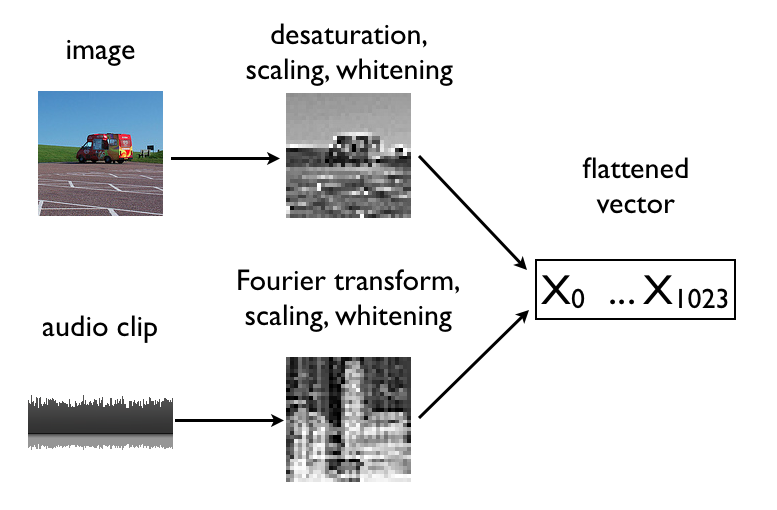
\includegraphics[width=6in]{data_prep}
\caption{The data from both sensory modalities is prepared to present vectors of the same width to the learning algorithms.}
\end{figure}

\begin{figure}[p]
\centering
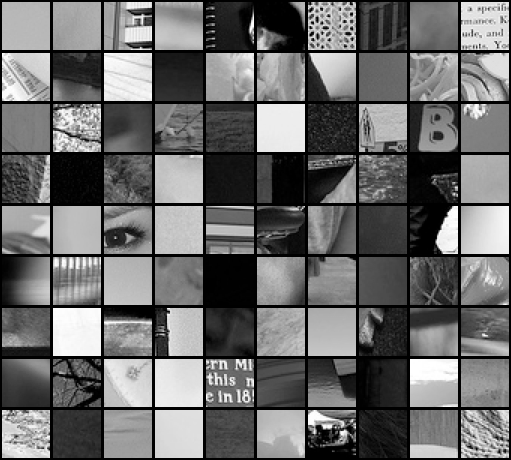
\includegraphics[width=6in]{patch_arrangment}
\caption{Patches sampled from the Flickr-1M dataset prior to whitening}
\end{figure}
	
	To the best of my knowledge there is no comparably rich, large, and well packaged sound dataset released under creative commons or in the public domain, so for this experiment I am using a collection of publicly aired talk-show broadcasts from which short clips are sampled and transformed into spectrograms of comparable dimensions to the image patches. The "patches" of spectrogram are 500 milliseconds long, divided into 32 time bins. They are also divided into frequency bins of 32 peak frequencies on a logarithmic scale with the lowest frequency peak being 50 hz and the highest being 10 khz. An equal number of samples were prepared from each sensory modality, images and sounds, and each datum is of the same dimensions, and is normalized in the same way. This way they can all be treated interchangeably, simplifying the code, and ensuring that any differences in learning between the two datasets are due to the differences in the content of their data, and not, for example, a different network topology for data of different dimensions.
	
	\subsection{Implementation}
	The SDA implementation I am using is based on the examples at [deep learning tutorials link] except I have modified the code to run on larger datasets and take better advantage of desktop GPU cards. The first autoencoder in the stack must have an input dimension of 1024, because that is the width of the input vectors. After that I have somewhat arbitrarily chosen additional layer widths of 500, 250, and 50. This topology was held constant throughout all experiments, and these dimensions are not unusual in the deep learning literature. My code is open source and available on github at [link]. 
	
	Both traditional neural networks and stacked denoising autoencoders take input examples as a real-valued vector and produce a real valued vector. They can be made to produce a classification at the output by assigning one class to each output level node and taking the maximally activated node as the most probably class for any given example, but in this experiment, because labeled data was unavailable, reconstruction error was used as a measure of learning performance. This means that input vectors are transformed via a stack of encoders, to the 32 unit hidden code, and then back through the decoders into a 1024 unit reconstruction of the input. This reconstruction is compared to the original, to obtain the reconstruction error.
	
	The control model is initialized as a multi-layered denoising autoencoder with random weights and the same topology as the experimental model trained using greedy-layer-wise pre-training (GLWPT). The primary difference between them is the way they are trained. When the experimental model is training on the first sensory modality, it will undergo greedy, layer-wise pre-training, meaning that it will begin with only one layer, treated as a stand-alone denoising autoencoder, and that encoder's (and decoder's) weights will be optimized to reduce the mean squared reconstruction error, using stochastic gradient decent. Periodically, the next denoising autoencoder in the pre-defined topology will be added and the network will begin minimizing that layer's reconstruction error instead. Once the network reaches the half-way point, greedy layer-wise pre-training stops and the network begins the fine-tuning phase, on opposite sensory modality. The fine tuning phase consists of assembling the weights into one large multi-layered denoising autoencoder, and minimizing it's complete reconstruction error from beginning to end. The training procedure used for the control model is identical to the fine tuning step of the experimental model.
	
	\subsection{Measuring neuro-plasticity}
	For each type of training method (SDA trained with GLWPT, and without)  a comparison will be made between networks trained on strictly one kind of data, and networks that have been "re-assigned" to a new type of data partway though training (multi-modal), The single modality model is relatively  straightforward, it is just trained normally and only images or only sound patches are used as input examples. The multi-modal model will train with examples from images, and then switch to sound, and since doing one of these last gives it an advantage, another model will be trained with sound first, then images.
	So, to summarize, there are two types of training procedure (with GLWPT and without) there are two experimental groups (single modality, and multiple modality) and within the multi-modal experimental group, there must be two experiments to control for the advantage given by training order (sound or images first) this gives 6 total models trained, as tabulated below.
	
\begin{figure}[p]
\centering
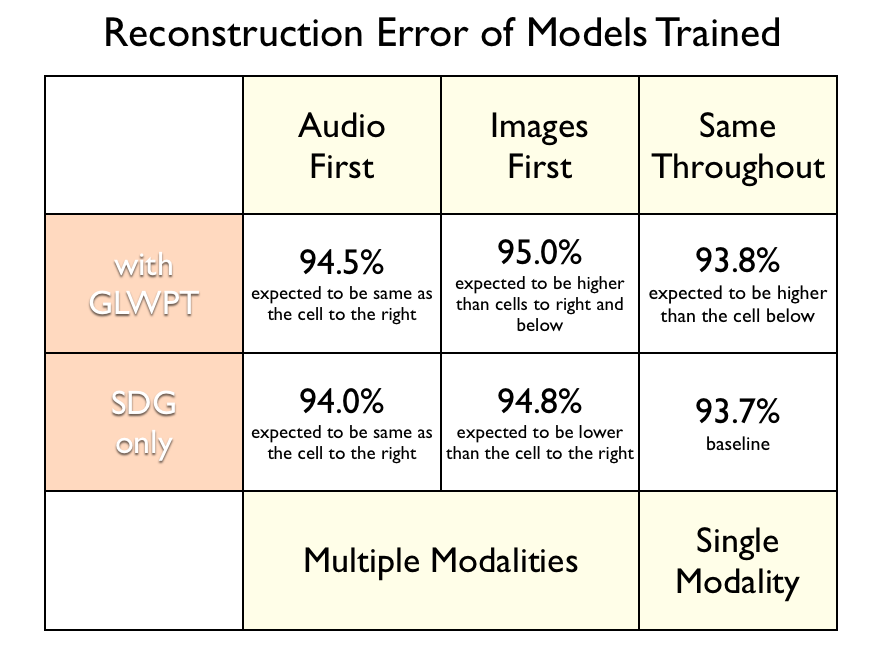
\includegraphics[width=6in]{table_of_models}
\caption{The reconstruction error of test examples for each experimental model after a total of 1 million training epochs each. }
\end{figure}

	The amount of additional training epochs needed by the single-modality model to catch up with the multi-modal model indicates how comparatively more valuable the re-assigned model's "incorrect" weights were vs. the random weights of the single-type model. \textbf{The magnitude of this number for the SDA experiment is expected to be larger than for the NN experiment because a hierarchical model which has discovered abstract features should be better prepared to re-use those features to represent new information.}
	
\section{Results and Conclusion}
	\subsection{Experimental results}
		The multi-modal SDAs trained with greedy layer-wise pre-training were able to achieve a [fill in] re-construction error on the final sensory modality vs. the SDA without GLWPT. This indicates that they are... 
		
		Similar: pre-training on the other sensory modality is just as good as pre-training on the correct sensory modality. They are statistically similar enough that pre-training does not pick up on the fine differences.
		Worse: it hinders the performance vs. no pre-training. this would be unlikely, but it would indicate that somehow pre-training is especially sensitive to initial conditions while plain SGD is not.
		Better: it gives the SGD a more general head-start which allows it to ultimately settle into a more optimal minimum.
	
	\subsection{Conclusion}
	This is but one simple measurement that is analogous to neuro-plasticity, But in the brain, plasticity is far more complicated and involves both modification of weights, and the alteration of the presence of network links and neurons. Likely, other unknown factors and limitations are involved as well. However, these experiments indicate that a hierarchical representation alone is sufficient to allow and improved level of plasticity. 

\end{doublespacing}

%MFLICKR Dataset
\nocite{huiskes08}

\singlespacing
\bibliographystyle{plain}
\bibliography{machine_learning_bibliography}



\end{document}






